 % !TEX TS-program = pdflatex
% !TEX encoding = UTF-8 Unicode

\documentclass[slidetop,11pt,table]{beamer}

%\usepackage[french]{babel}
%\usepackage[T1]{fontenc}
\usepackage[utf8]{inputenc}

\usepackage{float}
\usepackage{caption}
\usepackage{ifthen}

%\usetheme{Warsaw}
\usecolortheme{beaver}

% figures for both slides and article (Makefile coming soon ?)

\usepackage{tikz}
\usetikzlibrary{arrows.meta}
\tikzset{
  hwblock/.style={draw, rectangle, rounded corners=.3, very thick, fill=black!5, font=\sf, minimum height=5ex},
  hwbus/.style={very thick,>=stealth},
  hwwire/.style={thick,>=stealth},
  hwword/.style={draw, rectangle, minimum height=3ex},
  bitwidth/.style={font=\scriptsize,midway,right}
}

\newcommand{\figVonNeumann}{
  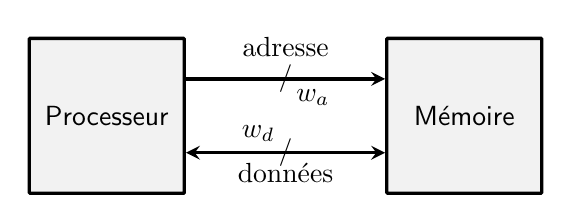
\begin{tikzpicture}
    \node[hwblock, minimum width=13ex,minimum height=13ex] (p) at (0,0)  {Processeur} ;
    \node[hwblock, minimum width=13ex,minimum height=13ex] (m) at (30ex,0)  {Mémoire} ;
    \draw[hwbus,->] (p.25) -- (m.155) node[midway,above=1ex]{adresse} node[midway]{/} node[midway, below right]{$w_a$};
    \draw[hwbus,<->] (p.335) -- (m.205) node[midway,below]{données} node[midway]{/} node[midway, above left]{$w_d$};
  \end{tikzpicture}
}

\newcommand{\proco}{
  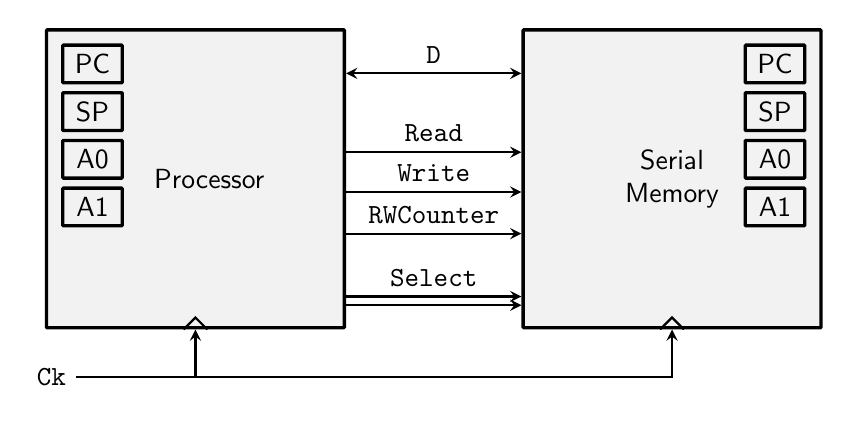
\begin{tikzpicture}
    \node[hwblock, minimum width=25ex,minimum height=25ex] (p) at (-10ex,0)  {~~~Processor} ;
%    \draw  (p) ++(0,-10ex)  node {} ;
    \node[hwblock, minimum width=25ex,minimum height=25ex, align=center] (m) at (30ex,0)  {Serial\\ Memory} ;
    
    \draw (p.north west)  ++(4ex,-3ex)  node[hwblock,minimum height=3ex,minimum width=5ex]{PC} ;
    \draw (p.north west)  ++(4ex,-7ex)  node[hwblock,minimum height=3ex,minimum width=5ex]{SP} ;
    \draw (p.north west)  ++(4ex,-11ex)  node[hwblock,minimum height=3ex,minimum width=5ex]{A0} ;
    \draw (p.north west)  ++(4ex,-15ex)  node[hwblock,minimum height=3ex,minimum width=5ex]{A1} ;
    
    \draw (m.north east)  ++(-4ex,-3ex)  node[hwblock,minimum height=3ex,minimum width=5ex]{PC} ;
    \draw (m.north east)  ++(-4ex,-7ex)  node[hwblock,minimum height=3ex,minimum width=5ex]{SP} ;
    \draw (m.north east)  ++(-4ex,-11ex)  node[hwblock,minimum height=3ex,minimum width=5ex]{A0} ;
    \draw (m.north east)  ++(-4ex,-15ex)  node[hwblock,minimum height=3ex,minimum width=5ex]{A1} ;

    \draw[hwwire,<->] (p.35) -- (m.145) node[midway,above]{\texttt{D}};

    \draw[hwwire,->] (p.10) -- (m.170) node[midway,above]{\texttt{Read}};
    \draw[hwwire,->] (p.355) -- (m.185) node[midway,above]{\texttt{Write}};
    \draw[hwwire,->] (p.340) -- (m.200) node[midway,above]{\texttt{RWCounter}};
    \draw[hwwire,->] (p.322) -- (m.218) node[midway,above]{\texttt{Select}};
    \draw[hwwire,->] (p.320) -- (m.220) node[midway,above]{};
    \draw[hwwire,<-] (m.south) -- ++(0,-4ex) -- ++(-50ex,0) node[left]{\texttt{Ck}};
    \draw[hwwire,<-] (p.south) -- ++(0,-4ex);
    \draw[hwwire,-] (p.south)  ++(-1ex, 0) -- ++(1ex,1ex) -- ++(1ex,-1ex); % horloge
    \draw[hwwire,-] (m.south)  ++(-1ex, 0) -- ++(1ex,1ex) -- ++(1ex,-1ex); % horloge
  \end{tikzpicture}
}

\newcommand{\progex}{
  \begin{tabular}{llll}
    \textrm{étiquette} & \textrm{mnémonique} & \textrm{encodage initial} & \textrm{encodage Huffman de l'opcode} \\
    \hline
    
         & leti	r0 17        & 0111 000 1000010001 & 100 000 1000010001 \\
         & leti	r1 42        & 0111 001 1000101010 & 100 001 1000101010 \\
         &                   &                     &                    \\
				 & leti	r2 0				 & 0111 010 00				 & 100 010 00       	\\
nonzero: & shift	right r0 1 & 1000 1 000 1				 & 00 1 000 1       	\\
				 & jumpif	nc next		 & 1011 101 000001010	 & 01 101 000001010 	\\
				 & add2	r2 r1				 & 0000 010 001				 & 1010 010 001     	\\
next:		 & shift	left r1 1	 & 1000 0 001 1				 & 00 0 001 1       	\\
				 & cmpi	r0 0				 & 0101 000 00				 & 11 000 00        	\\
				 & jumpif	nz nonzero & 1011 001 010111011	 & 01 001 011000101 	\\
         &                   &                                          \\
loop:    & jump	loop         & 1010 011110011      & 10110 011110010    \\
  \end{tabular}
}

\newcommand{\prefree}{
  \begin{tabular}{|l||l||l||ll|}
    \hline
    \emph{addr}&  \emph{const} & \emph{shiftval} & \emph{size}& \\
    adresses, déplacements & constantes ALU & constantes de shift & tailles     & \\
    \hline
    0 + 8 bits               & 0 + 1 bit      & 0 + 6 bits          & 00 : 1 bit &  01: 4 bits  \\ 
%    \hline         
    10 + 16 bits             & 10 + 8 bits    & 1  (constante 1)    & 100: 8 bits& 101: 16 bits \\
%    \hline                  
    110 + 32 bits            & 110 + 32 bits  &                     & 110: 32 bits &  \\
%    \hline                  
    111 + 64 bits            & 111 + 64 bits  &                     & 111: 64 bits &\\
    \hline
  \end{tabular}
}

\newcommand{\benchmark}{
    \begin{tabular}{|r||c|c|c||c|c|c|c|c||c|}
    \hline
    & \multicolumn{3}{c||}{taille du programme} & \multicolumn{6}{c|}{bits échangés à l'exécution}                    \\
    \hline

    
    benchmark      & instr     & bits       & BPI         & prog    & data R  & data W  & counters & branch  & total      \\
    \hline
    \hline
    binmult~~~I    & 10        & 125        & 12.5        & 89.4\%  &         &         &          & 10,6\%  & 415        \\
     H             &           & 113        & 11.3        & 85.5 \% &         &         &          & 14.5 \% & 373        \\
    \emph{ msp430} & \emph{10} & \emph{192} & \emph{19.2} & --      & --      & --      & --       & --      & \emph{960} \\
    \hline
    \hline
    matmul~~~I     & 112       & 1632       & 14.6        & 80.4 \% & 5.0 \%  & 2.6 \%  & 0.3 \%   & 11.8 \% & 1.72e8     \\ 
     (dense)~  H   & 112       & 1817       & 16.2        & 75.4 \% & 5.6 \%  & 2.9 \%  & 0.3 \%   & 15.9 \% & 1.54e8     \\ 
    \hline
    matmul~~~I     & 112       & 1632       & 14.6        & 55.3 \% & 23.3 \% & 12.1 \% & 1.2 \%   & 8.0 \%  & 3.68e7     \\ 

    (sparse)~ H & 112 & 1613 & 14.4  & 52.1 \% & 25.2 \% & 13.1 \% & 1.3 \% & 8.3 \% & 3.41e7\\ 

    \hline
    \hline
    Chip8~~~I     & 768 & 14155 & 18.4 &  64.3 \% & 10.4 \% & 9.7 \% & 7.5 \% & 8.1 \% & 1.068e8       \\
     H    & 768 & 13699 & 17.8 & 63.1 \% & 10.7 \% & 9.9 \% & 7.7 \% & 8.6 \% & 1.063e8\\ 
    \hline
  \end{tabular}
}

\title{Une architecture minimisant les échanges\\ entre processeur et mémoire}
\author{Florent de Dinechin, Maxime Darrin, Antonin Dudermel, Sébastien Michelland, Alban Reynaud}
\date{}

\begin{document}

\frame{\titlepage}

%\frame{\tableofcontents}

\begin{frame}{Architecture de Von Neumann}
  \begin{figure}[b]
    \begin{center}
      \figVonNeumann{false} % sans le PC
    \end{center}
    %\caption{Une machine de von Neumann.}
%    \label{fig:mvn} \index{von Neumann}\index{machine de von Neumann}
  \end{figure}
  Cycle de von Neuman:
  \begin{enumerate}
  \item lire l'instruction courante
  \item l'exécuter
  \item passer à l'instruction suivante et retourner en 1
  \end{enumerate}
\end{frame}


\begin{frame}{Architecture de Von Neumann}
  \begin{figure}[b]
    \begin{center}
      \figVonNeumann{true}
    \end{center}
    %\caption{Une machine de von Neumann.}
%    \label{fig:mvn} \index{von Neumann}\index{machine de von Neumann}
  \end{figure}
  Cycle de von Neuman:
  \begin{enumerate}
  \item lire l'instruction à l'adresse PC, et incrémenter PC
  \item exécuter cette instruction
    \only<2->{
      \begin{itemize}
      \item faire un calcul
      \item ou lire depuis la mémoire
      \item ou écrire en mémoire
      \item ou changer la valeur de PC
      \end{itemize}
    }
   
  \item retourner en 1
  \end{enumerate}
\end{frame}



\begin{frame}[fragile]{Sur le fil de données, il passe surtout du programme}
\begin{verbatim}
  ADDRESS   CODE           (IN READABLE FORM) 
    312c:	  3a40 1100      mov	#17,	r10	
    3130:	  7b40 2a00      mov	#42,	r11	
    3134:	  0c43       	   clr	r12		

loop:
    3136:	  0a10       	   rrc	r10		
    3138:	  0128       	   jnc	$+4      
    313a:	  0c5b       	   add	r11,	r12	
bit_is_zero:
    313c:	  0b5b       	   rla	r11		
    313e:	  0a93       	   tst	r10		
    3140:	  fa23       	   jnz	$-10     	

eternal_loop:
    3142:	  ff3f       	   jmp	$+0      	
\end{verbatim}
\end{frame}


\begin{frame}{Les questions qu'on se pose lorsqu'on conçoit un processeur}
  \begin{itemize}
  \item Quelles tailles pour $w_a$ et $w_d$
  \item Quelles sont les instructions les plus puissantes qu'on peut encoder en $w_d$ bits ?
  \item Quelles opérandes on encode et comment?
    
  \item Permet-on qu'une instruction occupe plusieurs mots?
  \item Permet-on plusieurs instructions par mots?
  \item ...
    
  \end{itemize}
\end{frame}

\begin{frame}{Le cours ASR1 au dept. info. de l'ENS-Lyon}
  \begin{itemize}
  \item Se poser ces questions
  \item Définir une architecture
  \item Écrire un simulateur et un programme assembleur
  \item Écrire plein d'assembleur
  \end{itemize}
  Tous les ans une règle du jeu différente 
\end{frame}




\begin{frame}{La règle du jeu de cette année}
Données et instructions de taille variable au bit près
  \begin{itemize}
  \item prétexte: minimiser la quantité d'information qui passe sur les bus
    \begin{itemize}
    \item donc l'énergie, mais en fait c'est un mensonge
    \end{itemize}
  \item objectif numéro 1: un jeu d'instructions universel
  \item objectif numéro 2: un jeu d'instructions optimisé
  \end{itemize}
  
\end{frame}




\begin{frame}{L'interface processeur-mémoire proposée}
  \begin{figure}[b]
    \begin{center}
      \scalebox{0.8}{\proco}
    \end{center}
  \end{figure}
  \begin{itemize}
  \item 6 fils seulement entre processeur et mémoire
  \item les données passent en série sur \texttt{D}
  \item la mémoire est adressable par bit
  \item les adresses sont implicites:
    \begin{itemize}
    \item 4 compteurs auto-incrémentés, et dupliqués
    \item les deux bits \texttt{Select} déterminent le compteur utilisé
    \end{itemize}
  \end{itemize}
\end{frame}




\begin{frame}{Jeu d'instruction}
  \begin{itemize}
  \item c\o eur de processeur classique: 32 ou 64 bits, 8 registres
  \item instructions à 0, 1, 2, 3, ou 4 opérandes, sans se poser de question
  \item code opération en premier (détermine combien d'opérande), suivi des opérandes
  \item registres toujours sur 3 bits mais constantes (et adresses) de taille variable
  \end{itemize}
\end{frame}



\begin{frame}{Un exemple}{multiplication entière}
  \begin{center}
    \tt\small
    \begin{tabular}{llll}
    \textrm{étiquette} & \textrm{mnémonique} & \textrm{encodage}\\
    \hline
    
				 & leti	r0 17				 & 0111 000 1000010001 \\
				 & leti	r1 42				 & 0111 001 1000101010 \\
				 &									 &										 \\
				 & leti	r2 0				 & 0111 010 00				 \\
nonzero: & shift	right r0 1 & 1000 1 000 1				 \\
				 & jumpif	nc next		 & 1011 101 000001010	 \\
				 & add2	r2 r1				 & 0000 010 001				 \\
next:		 & shift	left r1 1	 & 1000 0 001 1				 \\
				 & cmpi	r0 0				 & 0101 000 00				 \\
				 & jumpif	nz nonzero & 1011 001 010111011	 \\
				 &									 &										 \\
loop:		 & jump	loop				 & 1010 011110011			 \\
  \end{tabular}
\end{center}
Ici que des opcodes sur 4 bits, mais il y en a aussi sur 5 et 6 bits pour les instructions les moins utiles.
\end{frame}




\begin{frame}{Encodage \emph{prefix-free} des constantes}

  \begin{center}
    \begin{tabular}{|l||l|}
      \hline
      \emph{addr}&  \emph{const}  \\
      adresses, déplacements & constantes ALU    \\
      \hline
      0 + 8 bits               & 0 + 1 bit      \\ 
      % \hline         
      10 + 16 bits             & 10 + 8 bits    \\
      % \hline                  
      110 + 32 bits            & 110 + 32 bits  \\
      % \hline                  
      111 + 64 bits            & 111 + 64 bits   \\
      \hline
    \end{tabular}
    
    \begin{tabular}{|l||ll|}
      \hline
      \emph{shiftval} & \emph{size}& \\
      constantes de shift & tailles     &              \\
      
      0 + 6 bits          & 00 : 1 bit &  01: 4 bits  \\ 
      % 
      1  (constante 1)    & 100: 8 bits& 101: 16 bits \\
      % 
                      & 110: 32 bits &            \\
                      % 
                      & 111: 64 bits &             \\
      \hline
    \end{tabular}
  \end{center}
Un relecteur nous a fait remarquer que c'était un genre de Gamma-code ad-hoc.
\end{frame}



\begin{frame}{Spécificité: les accès mémoire}
  \begin{itemize}
  \item Instructions de lecture et écriture séquentielle de
    \emph{size} bits depuis/vers un registre
  \begin{itemize}
  \item avec \emph{padding} ou extension de signe
  \end{itemize}
  
\item transferts d'adresses:
  \begin{itemize}
  \item uniquement lors d'une rupture de séquentialité
  \item par une instruction spéciale: \texttt{setctr}
  \item l'adresse passe alors sur le fil \texttt{D} 
  \end{itemize}
\item Changement de PC (saut relatif, \texttt{call} absolu)
  \begin{itemize}
  \item même mécanisme
  \end{itemize}
\end{itemize}
Auto-critique: constantes en mémoire qui passent deux fois sur \texttt{D}.
\end{frame}



\begin{frame}{Quant à l'architecture...}
  Quelques automates reconnaisseurs interfacés sur une ALU et une boîte à registres classiques. 
  
  (seulement des bribes écrites en VHDL)

\end{frame}



\begin{frame}{Expériences et démos}
  \begin{itemize}
  \item Benchmarks (écrits à la main en assembleur):
    \begin{itemize}
    \item multiplication de deux entiers binaires
    \item produits de matrices denses (accès séquentiel) et creuses (accès aléatoire)
    \item émulateur de la machine virtuelle chip8
    \end{itemize}
  \item Mesure de la taille du code et du nombre de bits échangés à l'exécution
  \end{itemize}

  Et pour savoir si on est loin de l'optimal:
  \begin{itemize}
  \item Ré-encodage a-postériori des opcodes par un encodage
    optimal (Huffman)
  \end{itemize}

\end{frame}





\begin{frame}{Benchmark}{Nombre de bits par instruction}
    \centering
    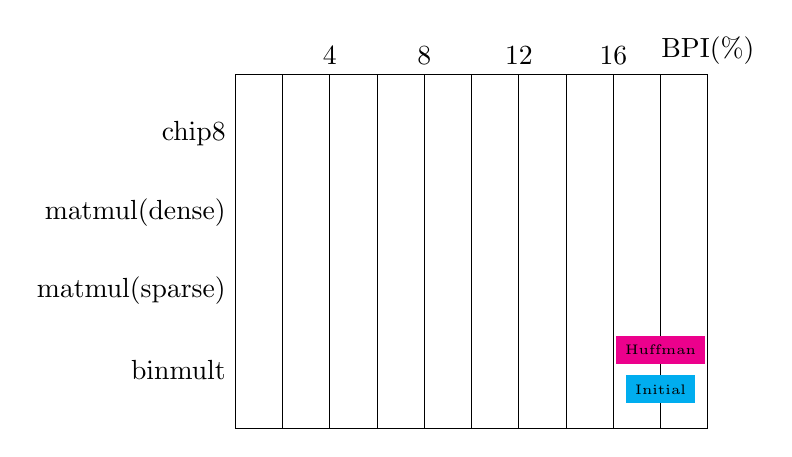
\begin{tikzpicture}[xscale = 0.3, yscale = 0.5]
      \draw(0,0)grid[xstep=2,ystep=9] (20,9);
      \draw[line width=4mm, color=magenta, yshift=-1mm] plot[xcomb] file {huffbpi.txt};
      \draw[line width=4mm, color=cyan, yshift=1mm] plot[xcomb] file {initbpi.txt};
      \foreach \x in {4,8,12,16} \draw(\x,9)node[above]{\x};
      \draw (20,9)node[above]{BPI(\%)}; 
      \foreach \n/\y in {binmult/1.5,matmul(sparse)/3.5,matmul(dense)/5.5,chip8/7.5} 
      \draw (0,\y) node [left] {\n};
      \draw (18,1) node[fill=cyan] {\tiny Initial};
      \draw (18,2) node[fill=magenta]{\tiny Huffman};
    \end{tikzpicture}
\end{frame}

\begin{frame}{Benchmark}{Nobre de bits échangés à l'exécution}
    \centering
    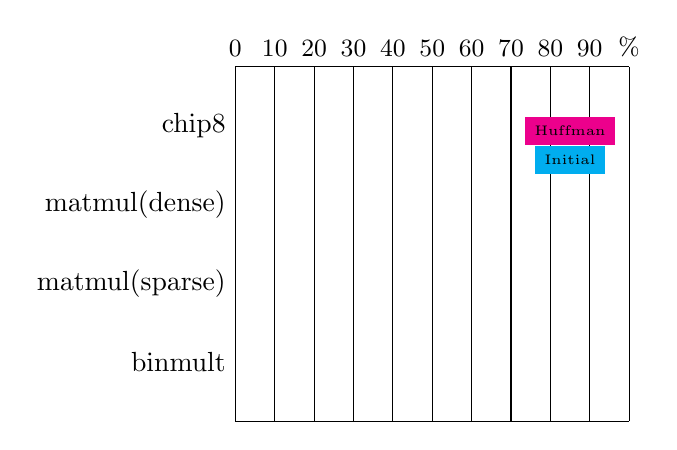
\begin{tikzpicture}[xscale=0.05,yscale=0.5]
      \draw(0,0)grid[xstep=10,ystep=9] (100,9);
      \draw[line width=4mm, color=magenta, yshift=-1mm] plot[xcomb] file {huffprgm.txt};
      \draw[line width=4mm, color=cyan, yshift=1mm] plot[xcomb] file {initprgm.txt};
      \foreach \x in {0,10,...,90} \draw(\x,9)node[above]{\small\x};
      \draw (100,9)node[above]{\small \%}; 
      \foreach \n/\y in {binmult/1.5,matmul(sparse)/3.5,matmul(dense)/5.5,chip8/7.5} 
      \draw (0,\y) node [left] {\n};
      \draw (85,7) node[fill=cyan,below] {\tiny Initial};
      \draw (85,7) node[fill=magenta,above]{\tiny Huffman};
      
    \end{tikzpicture}
\end{frame}

% \begin{frame}
%   \frametitle{Bibliographie}
%   \bibliographystyle{plain}
%   \bibliography{../biblio}
% \end{frame}

\begin{frame}{Conclusion}
  \begin{itemize}
  \item Le gros des bits échangés à l'exécution sont des bits de programmes
    \begin{itemize}
    \item cache dédié dans les vrais processeurs
    \end{itemize}
  \item Encodage d'un processeur 64 bits plus compact que le MSP430 16 bits, mais pas tant que cela
    \begin{itemize}
    \item MSP430 et ARM ont un très bon encodage des instructions les plus courantes
    \item on paye le prix des préfixes d'auto-description
    \end{itemize}
  \item Quelques challenges
    \begin{itemize}
    \item assymétrie entre \texttt{pop} et \texttt{push}
    \end{itemize}
  \item Comment grater plus?
    \begin{itemize}
    \item encodage des opcodes: sans doute peu à gagner.
    \item moins de 3 bits par registres ? (accumulateur implicite, fenêtre de registres)
    \end{itemize}
  \end{itemize}

\end{frame}



\begin{frame}{Et une vraie question}
  Existe-t-il un contexte dans lequel ceci est utile en pratique?
  \begin{itemize}
  \item Cette interface limite la fréquence d'horloge bien en dessous des 100 MHz.
  \item ... et chaque instructions prend en moyenne 12-20 cycles
  \item En terme de consommation:
    \begin{itemize}
    \item il faut compter les transitions, \emph{y compris sur
        l'horloge}.
  
  \item a cause du lien série, les transitions économisées sur le bus d'adresse sont remplacées par  des transitions d'horloge. 
  \end{itemize}
  
\item En d'autre termes le marché est celui de
  \begin{itemize}
  \item systèmes ayant besoin de mémoire discrète (donc beaucoup de mémoire),  
  \item mais pas de haute-performance...
\end{itemize}

  \end{itemize}

  
\end{frame}

\end{document}